\documentclass[tikz,border=3pt]{standalone}
\usepackage[utf8]{inputenc}
\usepackage[T1]{fontenc}
\usepackage{lmodern}
\renewcommand{\familydefault}{\sfdefault}
\usepackage{sansmath}\sansmath
\usepackage{pgfplots}\pgfplotsset{compat=1.18,/pgf/number format/use comma,/pgf/number format/1000 sep={.}}
\usetikzlibrary{arrows.meta,calc,positioning,decorations.pathmorphing,patterns}
% paleta del sitio
\definecolor{nar}{HTML}{E8680C}\definecolor{narc}{HTML}{FFB35C}\definecolor{hielo}{HTML}{FFF3E8}
\definecolor{tinta}{HTML}{1D1D1F}\definecolor{gris}{HTML}{6E6E73}\definecolor{lila}{HTML}{7C5CF0}
\definecolor{azul}{HTML}{2F6FD6}\definecolor{menta}{HTML}{17A673}\definecolor{coral}{HTML}{E8342A}
\begin{document}
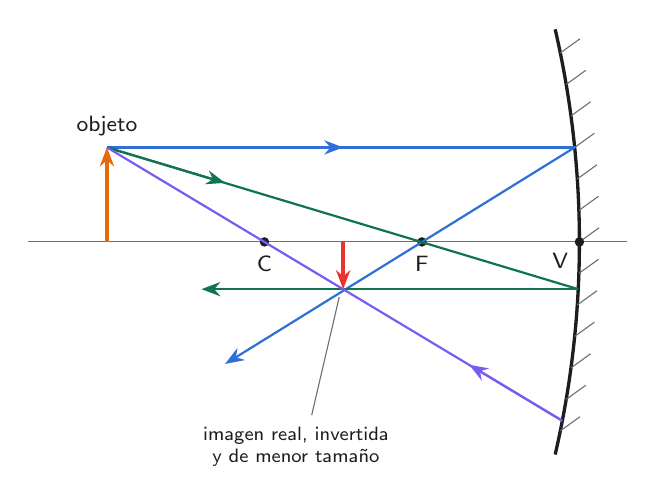
\begin{tikzpicture}[font=\footnotesize,>={Stealth[length=2.4mm]}]
\draw[gris] (-7,0) -- (0.6,0);
\draw[very thick,tinta,domain=-2.7:2.7,samples=60,smooth] plot ({-12+sqrt(144-\x*\x)},\x);
\foreach \y in {-2.4,-2.0,...,2.41} \draw[gris,thin] ({-12+sqrt(144-\y*\y)},\y) -- ++(0.25,0.18);
\foreach \x/\t in {-2/F,-4/C} {\fill[tinta] (\x,0) circle (0.06); \node[below,text=tinta] at (\x,-0.05) {\t};}
\fill[tinta] (0,0) circle (0.06); \node[below left,text=tinta] at (-0.02,-0.02) {V};

\draw[->,line width=1.6pt,nar] (-6,0) -- (-6,1.2) node[above,text=tinta] {objeto};
\draw[azul,thick] (-6,1.2) -- (-0.06,1.2); \draw[->,azul,thick] (-6,1.2) -- (-3,1.2);
\draw[->,azul,thick] (-0.06,1.2) -- (-4.5,-1.55);
\draw[menta!70!black,thick] (-6,1.2) -- (-0.015,-0.6); \draw[->,menta!70!black,thick] (-6,1.2) -- (-4.5,0.75);
\draw[->,menta!70!black,thick] (-0.015,-0.6) -- (-4.8,-0.6);
\draw[lila,thick] (-6,1.2) -- (-0.22,-2.27); \draw[->,lila,thick] (-0.22,-2.27) -- (-1.4,-1.56);
\draw[->,line width=1.6pt,coral] (-3,0) -- (-3,-0.6);
\node[text=tinta,align=center,font=\scriptsize] at (-3.6,-2.6) {imagen real, invertida\\y de menor tamaño};
\draw[gris,thin] (-3.05,-0.7) -- (-3.4,-2.2);
\end{tikzpicture}
\end{document}
